% !TEX root = ../../../Lazcorreta.Tesis.tex
\ABIERTO
\borrar{Buen momento para hablar de lío de \datasets que hay, de que el primero que encontramos en FIMI no tenía metadatos y lo tratamos como todos puramente con \ARM hasta que descubrimos que era \verb"tipo II".}

Esta colección de datos ha sido utilizada para experimentar en muchas investigaciones y con propósitos y propuestas bien diferentes. En todas ellas se analiza utilizando el umbral de \soporte mínimo pese a sus reducidas dimensiones. El problema que presenta el uso de \soporte mínimo en este fichero reside en que un 23\% de sus ítems tienen soporte menor al 1\% -- aparecen en 812 \transacciones o menos -- con lo que este umbral provoca que en todas las investigaciones revisadas no se obtenga información sobre al menos 27 ítems de los 119 presentes en el \dataset. Al usar estas colecciones como meros contenedores de \transacciones para demostrar la eficiencia de nuevos algoritmos los investigadores renuncian a obtener información de mayor calidad, si se pudieran repetir todos los experimentos realizados utilizando la información descrita en este capítulo cambiarían notablemente todos los resultados y en muchos casos se podría llegar a conclusiones que van más allá del objetivo de esta tesis.

%TODO: Aunque lo he descubierto en enero de 2016, WangWong-FromAssociationToClassificationInferenceUsingWeightOfEvidence-2003 me da mucho juego a rebatir las afirmaciones que hace usando el soporte como medida "intermedia" de calidad o de interés. Estudiarlo mejor, además voy a usar su notación.
\citet{WangWong-FromAssociationToClassificationInferenceUsingWeightOfEvidence-2003} presentan el \emph{peso de la evidencia} como una nueva medida para calibrar el interés de una \ar. Su trabajo se basa en la medida de \emph{información mutua}~\citep{no-la-tengo-y-no-la-consigo-1974} que a su vez se basa en el \soporte de las reglas en estudio. La argumentación y notación utilizada en este artículo ha sido muy útil para la redacción de esta tesis, de hecho el término \emph{evidencia empírica} representa al concepto que en principio denominamos \emph{\ar determinista}.

\citet{Borgelt-EfficientImplementationsOfAprioriAndEclat-2004} usa \mushroom para mostrar la eficiencia de sus implementaciones de \apriori y \algoritmo{Eclat} con un \soporte mínimo absoluto fijado entre 200 y 1\,000 \transacciones (equivalente a un \soporte relativo del 2.46\% y 12.31\% respectivamente), prescindiendo de gran parte de la información contenida en el \dataset.

\citet{Suzuki-DiscoveringInterestingExceptionRulesWithRulePair-2004} busca reglas inesperadas en su investigación por lo que tendrá que lidiar con soportes bajos. Apunta que \mushroom puede tratarse sin \soporte mínimo pero su experimento tarda 80 días en dar resultados por lo que opta por prescindir de parte de la información disponible en el fichero.

\citet{ThabtahCowlingHammoud-ImprovingRuleSorting-2006} hacen énfasis en la utilidad teórica del \soporte mínimo:
\begin{quote}
Given a history or a training data set, the task of an AC algorithm is to discover the complete class association rules with significant supports and high confidences (attributes values that have frequencies above user specified constraints, denoted by minimum support (minsup) and minimum confidence (minconf) thresholds).
\end{quote}

\citet{LuoZhang-AnEfficientFIMAlgorithm-2007} usan \mushroom para probar su nuevo algoritmo, \emph{DiffsetHybrid}, con el que aseguran reducir las necesidades de uso de memoria. A pesar de ello utilizan \soportes mínimos del 10\%, 20\% y 30\%.

\citet{WangXinCoenen-MiningEfficientlySignificantCAR-2008} analizan \mushroom con un 1\% de \soporte mínimo a pesar de reducir el número de ítems a considerar de los 119 del \dataset original a 90, con lo que ya reducen las dimensiones del problema original, perdiendo incluso algo más de información que no está demostrado que sea más o menos valiosa que la información recogida en el \dataset original.

\citet{JinMcCallenBreitbartFuhryWang-EstimatingTheNumberOfFIInLargeDB-2009} hacen un estudio sobre el umbral de \soporte mínimo adecuado para este fichero utilizando valores para este umbral entre el 8\% y el 40\%.

\citet{LiChen-MiningNonDerivableFIOverDataStream-2009} califican a \mushroom como una colección densa y con alta correlación, lo que según los autores dificulta su estudio con niveles bajos de \soporte mínimo.

\citet{LiZhang-MiningMaximalFIOnGraphicsProcessors-2010} proponen el uso de "`Maximal Frequent Itemsets"' como una representación compacta de los \itemsets frecuentes contenidos en un \dataset, con lo que se necesita menos memoria para su almacenamiento y se puede aliviar el \dilemaIR. A pesar de ello también recurren al uso de \soporte mínimo en el análisis de esta colección de datos.

\citet{HLeon-DesarrolloDeClasificadoresBasadosEnCAR-2011} utiliza esta colección de datos, con 90 ítems distintos en lugar de los 119 originales. Propone la medida de calidad \emph{Netconf} como sustituto del \soporte mínimo, que fijan en el 1\% para hacer comparables sus aportaciones con las de otros investigadores.

\citet{MalikRaheja-ImprovingPerformanceOfFrequentItemsetAlgorithm-2013} y \citet{RituArora-IntensificationOfExecutionOfFrequentItemSetAlgorithms-2014} presentan el mismo trabajo bajo diferentes títulos. Utilizan esta colección de datos para comparar la eficiencia de tres algoritmos de \ARM aplicando \soporte mínimo del 10\%, 20\%\ldots 100\%.

\citet{SahooKumarGoswami-AnAlgorithmForMiningHighUtilityClosedItemsetsAndGenerators-2014} argumentan que el uso de \soporte-\confianza está sobrevalorado ya que estas medidas son puramente estadísticas y no aportan información de utilidad real de los \itemsets encontrados en el \dataset. Incorporan una medida de utilidad, asignada por el investigador, que se completa con el \soporte de los ítems en el \dataset. No indican qué valor asignan al \soporte mínimo pero siguen utilizándolo y, con ello, renunciando a parte de la información presente en la colección de datos a pesar de sus reducidas dimensiones.

\begin{wrapfigure}{o}{0.22\textwidth}
  \centering
  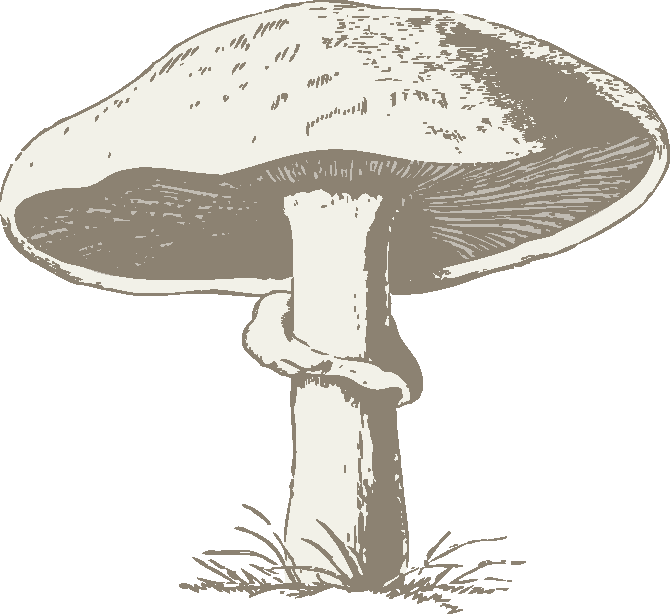
\includegraphics[width=.22\textwidth]{johnny_automatic_mushroom.pdf}
	\caption{Seta (\mushroom)}
	\label{fig:Seta}
\end{wrapfigure}
Al revisar la documentación sobre \mushroom\footnote{Ilustración obtenida en {\scriptsize\url{https://openclipart.org/detail/900/two-mushrooms-by-johnny_automatic}}} pudimos plantear mejor el problema que queríamos resolver, encontrar todas las \ARs presentes en un fichero "`pequeño"' que presenta estas características. En \urlConNotaAlPie{https://archive.ics.uci.edu/ml/datasets/Mushroom}{UCI - Machine Learning Repository} describen su origen como
\selectlanguage{english}
\begin{quote}
   Mushroom records drawn from The Audubon Society Field Guide to North American Mushrooms (1981). G. H. Lincoff (Pres.), New York: Alfred A. Knopf 
\end{quote}
\selectlanguage{spanish}

%TODO: Esta línea aparece con demasiado margen
%\noindent 
Describen brevemente el contenido del fichero, indicando que se trata de setas clasificadas como comestibles o venenosas (primer valor de cada fila).
\selectlanguage{english}
\begin{quote}
\label{cita:incertidumbre-suprimida-en-mushroom}
   This data set includes descriptions of hypothetical samples corresponding to 23 species of gilled mushrooms in the Agaricus and Lepiota Family (pp. 500-525). Each species is identified as definitely edible, definitely poisonous, or of unknown edibility and not recommended. This latter class was combined with the poisonous one. The Guide clearly states that there is no simple rule for determining the edibility of a mushroom; no rule like ``leaflets three, let it be'' for Poisonous Oak and Ivy.
\end{quote}
\selectlanguage{spanish}
\noindent Y explican los valores que puede tomar cada uno de los atributos.
\selectlanguage{english}
\begin{quote}
   \footnotesize
   1. cap-shape: bell=b, conical=c, convex=x, flat=f, knobbed=k, sunken=s
   
   2. cap-surface: fibrous=f, grooves=g, scaly=y, smooth=s

   3. cap-color: brown=n, buff=b, cinnamon=c, gray=g, green=r, pink=p, purple=u, red=e, white=w, yellow=y

   4. bruises?: bruises=t, no=f

   5. odor: almond=a, anise=l, creosote=c, fishy=y, foul=f, musty=m, none=n, pungent=p, spicy=s

   6. gill-attachment: attached=a, descending=d, free=f, notched=n

   7. gill-spacing: close=c, crowded=w, distant=d

   8. gill-size: broad=b, narrow=n

   9. gill-color: black=k, brown=n, buff=b, chocolate=h, gray=g, green=r, orange=o, pink=p, purple=u, red=e, white=w, yellow=y

   10. stalk-shape: enlarging=e, tapering=t

   11. stalk-root: bulbous=b, club=c, cup=u, equal=e, rhizomorphs=z, rooted=r, missing=?

   12. stalk-surface-above-ring: fibrous=f, scaly=y, silky=k, smooth=s

   13. stalk-surface-below-ring: fibrous=f, scaly=y, silky=k, smooth=s

   14. stalk-color-above-ring: brown=n, buff=b, cinnamon=c, gray=g, orange=o, pink=p, red=e, white=w, yellow=y

   15. stalk-color-below-ring: brown=n, buff=b, cinnamon=c, gray=g, orange=o, pink=p, red=e, white=w, yellow=y

   16. veil-type: partial=p, universal=u

   17. veil-color: brown=n, orange=o, white=w, yellow=y

   18. ring-number: none=n, one=o, two=t

   19. ring-type: cobwebby=c, evanescent=e, flaring=f, large=l, none=n, pendant=p, sheathing=s, zone=z

   20. spore-print-color: black=k, brown=n, buff=b, chocolate=h, green=r, orange=o, purple=u, white=w, yellow=y

   21. population: abundant=a, clustered=c, numerous=n, scattered=s, several=v, solitary=y

   22. habitat: grasses=g, leaves=l, meadows=m, paths=p, urban=u, waste=w, woods=d
\end{quote}
\selectlanguage{spanish}

El fichero \mushroom\footnote{\scriptsize\url{https://archive.ics.uci.edu/ml/machine-learning-databases/mushroom/agaricus-lepiota.data}} original es un fichero de texto con 8\,124 líneas, de las que muestro aquí las tres primeras:
\begin{quote}
   \footnotesize
   p,x,s,n,t,p,f,c,n,k,e,e,s,s,w,w,p,w,o,p,k,s,u
   
   e,x,s,y,t,a,f,c,b,k,e,c,s,s,w,w,p,w,o,p,n,n,g
   
   e,b,s,w,t,l,f,c,b,n,e,c,s,s,w,w,p,w,o,p,n,n,m
\end{quote}

El fichero \mushroom\footnote{\scriptsize\url{http://fimi.ua.ac.be/data/mushroom.dat}} con el que llevo años trabajando está codificado de otro modo, conteniendo la misma información
\begin{quote}
   \footnotesize
   1 3 9 13 23 25 34 36 38 40 52 54 59 63 67 76 85 86 90 93 98 107 113
   
   2 3 9 14 23 26 34 36 39 40 52 55 59 63 67 76 85 86 90 93 99 108 114
   
   2 4 9 15 23 27 34 36 39 41 52 55 59 63 67 76 85 86 90 93 99 108 115
\end{quote}

Este modo de registrar información sobre los individuos de una población es muy habitual en todas las ciencias. Se determina qué \atributos se pueden medir, codificándolos mediante un número reducido de valores distintos y mutuamente excluyentes, se observa a un \emph{individuo} y se mide el valor que toma en cada uno de los \atributos seleccionados, obteniendo un conjunto de códigos. Ya apuntaban \citet{LiuHsuMa-IntegratingClassificationAndARM-1998} que este tipo de \datasets tienen más asociaciones que las clásicas \transacciones de \ARM pero también cabe destacar que las dimensiones de estos \datasets son menores, en general, que las de aquellos obtenidos por la "`cesta de la compra"' debido a que muchos individuos de la población producen la misma \transaccion y a que las características de los \atributos en estudio pueden presentar incompatibilidades que reducirán las asociaciones que podrían darse entre los diferentes códigos usados para su modelización.
